\section{Theorie}
\label{sec:Theorie}

Mit dem Geiger-Müller-Zählrohr kann $\alpha$-\;$\beta$- und $\gamma$ -Strahlung gemessen
werden, indem ein elektrischer Impuls erzeugt wird. Es ist besonders aufgrund seiner
einfachen Konstruktion und den geringen Ansprüchen an die Elektronik beliebt, obwohl es
einige Nachteile besitzt.

\subsection{Aufbau}


\begin{figure}
  \centering
  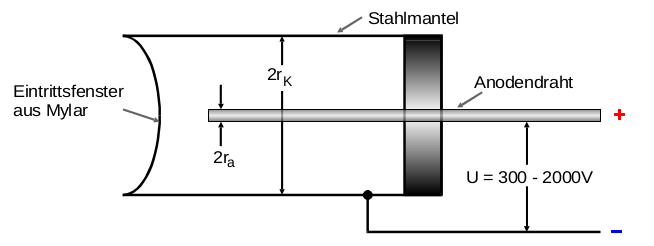
\includegraphics[width=8cm]{geiger.png}
  \caption{Das Geiger-Müller-Zählrohr}
  \label{fig:geiger}
  \cite{skript}
\end{figure}
Das Geiger-Müller-Zählrohr besteht aus aus einem positiv geladenem Anodendraht (Radius $r_a$) und
einem negativ geladenem Kathodenzylinder (Radius $r_k$).
Das innere Volumen ist mit einem Gasgemisch aus Argon und
Ethylalkohol gefüllt. Wird nun eine äußere Spannung angelegt bildet sich ein
radial symmetrisches Feld, die Feldstärke im Abstand $r$ wird durch
\begin{equation}
  E(r)=\frac{U}{r\ln(\frac{r_k}{r_a})}
\end{equation}
beschrieben. Die Beschleunigung eines geladenen Teilchens in diesem Feld
wächst also  mit $1/r$, also kann sie beliebig groß werden, wenn $r_a$ hinreichen
klein ist.
Tritt nun ein Teilchen in das Zählrohr ein, bewegt es sich so lange durch den
Gasraum, bis die gesamte Energie durch Ionisationsakte aufgebraucht ist.
Dabei ist die Anzahl der entstehenden Elektronen und positiven Ionen proportional
zur Energie des einfallenden Teilchens.
Die Vorgänge im Zählrohr hängen stark von der angelegten Spannung ab, daher werden
die folgenden Bereiche unterschieden.
\begin{figure}
  \centering
  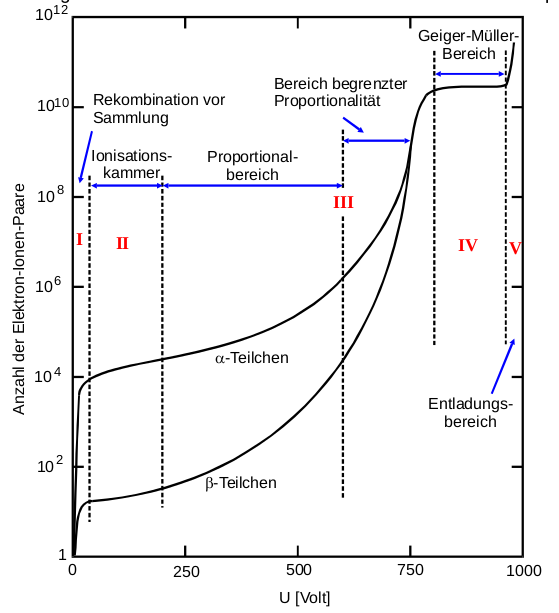
\includegraphics[height=6cm]{diagramm.png}
  \caption{Anzahl der Elektronen-Ionenpaare aufgetragen gegen die Spannung.}
  \label{fig:diagramm}
  \cite{skript}
\end{figure}

Bereich 1: Bei niedrigen Spannungen erreicht nur ein Teil der Strahlung den Anodendraht.
Der Rest geht durch Rekombination verloren.\\

Bereich 2: Hier sinkt die Rekombinationswahrscheinlichkeit ab, fast alle
Elektronen gelangen zum Anodendraht. Der nun fließende Strom ist proportional
zur Enegie und Intensität der einfallenden Teilchen. Geräte die mit dieser
Spannung arbeiten sind Ionisationskammern und stellen eine Vorstufe zum
Zählrohr dar. Aufgrund der geringen Ionisationsströme kann sie nur bei hohen
Strahlintensitäten eingesetzt werden.\\

Bereich 3: In diesem Bereich nehmen die Elektronen zwischen den Zusammenstößen mit
den Argon-Atomen genügend Energie auf, um die Gas-Atome durch Stoßionisation zu
ionisieren. Die so frei werdenden Elektronen werden ebenfalls beschleunigt und
lösen weitere Elektronen aus. So kommt es zu einer Lawine von ausgelösten
Elektronen, der Townsend-Lawine. Die Ladung $Q$ am Zählrohr pro einfallendes Teilchen ist
nun groß genug, um sie als Ladungsimpuls zu messen.
Dabei ist der Ladungsimpuls proportional zur Energie des Teilchens.
Dieses Zählrohr wird als Proportionalitätszählrohr bezeichnet und ist in der Lage
sowol Intensitäts-, als auch Energiemessungen durchzuführen.\\

Bereich 4: Dies ist der Auslösebereich, der Arbeitsbereich der Geiger-Müller-Zählrohrs.
Durch Elektronenstoß werden die Argon-Atome angeregt, wodurch UV-Photonen entstehen. Aufgrund
ihrer Ladungsneutralität können sie sich auch senkrecht zum Feld ausbreiten und die
Elektronen-Lawine ist nicht länger lokal beschränkt. Jetzt werden im gesamten
Zählrohrvolumen Elektronen ausgelöst. Die Ladung am Zählrohrdraht hängt jetzt von
dem Volumen des Zählrohres und der Spannung ab. Hier kann nur eine Intensitätsmessung, keine
Energiemessung vorgenommen werden. Da die Ladung aber so groß ist, ist kein großer
elektronischer Aufwand nötig um die Ladung nachuweisen.\\

\subsection{Totzeit und Nachentladung}
Die positiven Ionen halten sich aufgrund ihrer großen Masse lange im Gasraum auf, bis
sie zur Kathode wandern. Dadurch baut sich im Zählrohrvolumen eine positive
Raumladung auf, die das elektrische Feld abschirmt. Dadurch wird die Feldstärke
für eine Zeit $T$ so stark herabgesetzt, dass keine Stoßionisation mehr
möglich ist. Diese Zeit wird Totzeit genannt. Teilchen die in diesem Moment in das
Zählrohr einfallen werden also nicht registriet. Die positiv geladenen Ionen wandern dann
zum Zählrohrmantel, wo sie neutralisiert werden. Dann können neu einfallende Teilchen auch
wieder registriert werden. Die Ladungsimpulse $Q$ erreichen erst dann wieder ihre
ursprüngliche Höhe, wenn die Ionen vollständig neutralisiert sind, daher schließt sich an
die Totzeit die Erholungszeit $T_E$ an.

\begin{figure}
  \centering
  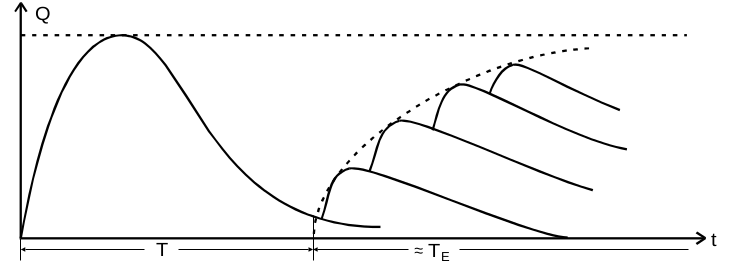
\includegraphics[width=8cm]{tot.png}
  \caption{Tot- und Erholungszeit einer Zählrohres.}
  \cite{skript}
\end{figure}

\subsubsection{Zwei-Quellen-Methode}
Mit der Zwei-Quellen-Methode kann die Totzeit eines Zählrohrers bestimmt werden.
Dazu werden zwei verschiedene Quellen benötigt. Die Zählrate der Quellen wird sowohl einzeln
als auch zusammen gemessen. Die in das Zählrohr eintretende Teilchenzahl wird dabei mit $N_W$
bezeichnet, während die tatsächlich registrierte Teilchenzahl mit $N_r$
bezeichnet wird. Für die in das Zählrohr eintretende Teilchenzahl ergibt sich die
Formel:
\begin{equation}
  N_W=\frac{N_r}{1-TN_r}.
  \label{eqn:n}
\end{equation}
Dabei ist $TN_r$ die Totzeit und $1-TN_r$ somit die messbereite Zeit.
Für die beiden Einzelmessungen $N_{W1}$, $N_{W2}$, als auch die Doppelmessung $N_{W1+2}$ ergibt sich somit aus
Gleichung \ref{eqn:n}:
\begin{equation}
  N_{W1}=\frac{N1}{1-TN_1}.
\end{equation}
Diese Formel gilt äquivalent für die anderen Messungen.
Einsetzen in die Beziehung $N_{W1+2}=N_{W1}+N_{W2}$ ergibt näherungsweise:
\begin{equation}
  T=\frac{N_1+ N_2- N_{1+2}}{2N_1 N_2}.
  \label{eqn:tot}
\end{equation}

\subsection{Nachentladung}
Treffen die Ionen auf den Zählrohrmantel könne sie dort Elektronen aus dem
Zylindermantel auslösen, da bei der Neutralisation genügend Energie frei wird
um die Austrittsarbeit für Elektronen aufzubringen. Diese Sekundärelektronen
durchlaufen das gesamte Zählrohrpotential und können eine erneute Zählrohrentladung
auslösen. Dadurch kommt es nach dem Durchgang eines einzelnen Teilchens zu mehreren zeitlich
versetzten Ausgangsimpulsen. Dieser Vorgang wird als Nachentladung bezeichnet.
Nachentladungen sind unerwünscht, da sie den Durchgang von ionisierenden Teilchen
vortäuschen. Um sie zu vermeiden werden Alkoholdämpfe zum Zählrohrgas hinzugegeben.
Die Ionen stoßen nun auf ihrem Weg zur Kathode mit den Alkoholmolekülen zusammen, wobei
diese ionisiert werden, da sie eine geringer Ionisierungsenergie besitzen.
Die Alkoholionen werden enfalls an der Kathode neutralisiert, doch wird die frei werdende
Energie zur Anregung von Schwingungen der Alkoholmoleküle verwendet.

\subsection{Die Charakteristik}
Die Charakteristik eines Zählrohres ergibt sich, indem sie Teilchenanzahl $N$ bei konstanter
Strahlungsintensität gegen die angelegte Spannung $U$ aufgetragen wird.
Der Auslösebereich setzt bei einer Spannung $U_E$ ein, der anschließende lineare Teil
heißt Plateau. Bei idealen Zählrohren ist der Plateausteigung Null.
Durch wenige Nachentladungen ist aber immer ein geringer Anstieg vorhanden.
Ein gutes Zählrohr ist ein einem langen Plateau mit geringem Anstieg zu erkennen.
Am Ende des Plateaus ist ein gewaltiger Anstieg zu beobachten, hier kann durch ein einziges
Teilchen eine Dauerentladung gezündet werden. Dieser Bereich der selbstständigen Gasentladung
kann das Zählrohr leicht zerstören.

\begin{figure}
  \centering
  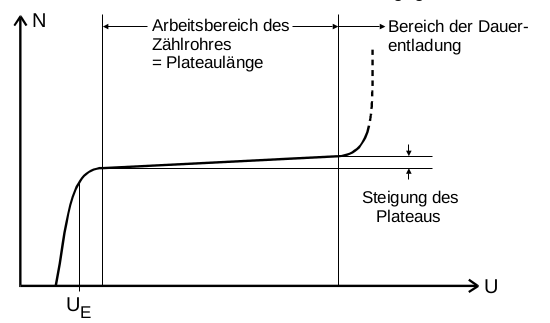
\includegraphics[height=6cm]{plateau.png}
  \caption{Charakteristik eines Zählrohres.}
  \cite{skript}
\end{figure}

\subsection{Ansprechvermögen}
Dies ist die Wahrscheinlichkeit, dass ein einfallendes Teilchen im Zählrohr
nachgewiesen wird. Aufgrund ihres hohen Ionisationsvermögens haben
$\alpha$- und $\beta$-Teilchen ein Ansprechvermögen von nahezu 100\%.
Dafür muss aber garantiert werden, dass die Teilchen in das Zählrohrvolumen gelangen.
Da $\alpha$- und $\beta$-Teilchen eine hohe Wechselwirkungswahrscheilichkeit mit Materie
haben, wird an einem Ende des Zählrohres ein Fenster aus einem Material mit
geringer Ordnungszahl verbaut, damit $\alpha$- und $\beta$-Teilchen in das Zählrohr eindringen
können. Solche Zählrohre werden Endfensterzählrohre genannt.
Das Ansprechvermögen für Photonen ist hingegen sehr gering. Deshalb kann das
Geiger-Müller-Zählrohr nur für Messungen hoher $\gamma$-Intensitäten sinnvoll
eingesetzt werden. Eine Ausnahme bilden die vergleichsweise niederenergetischen
Röntgen-Quanten, wenn ein schweres Füllgas wie z.B. Xeon verwendet wird.
